%% ============================================================
%% trossen_sim2real_ros — Technical Description
%% Suitable for inclusion in a thesis or technical paper.
%% Compile with: pdflatex -> bibtex -> pdflatex -> pdflatex
%% ============================================================
\documentclass[12pt, a4paper]{article}

\usepackage[utf8]{inputenc}
\usepackage[T1]{fontenc}
\usepackage{lmodern}
\usepackage[margin=25mm]{geometry}
\usepackage{amsmath, amssymb}
\usepackage{booktabs}
\usepackage{tabularx}
\usepackage{multirow}
\usepackage{graphicx}
\usepackage{listings}
\usepackage{xcolor}
\usepackage{hyperref}
\usepackage{caption}
\usepackage{subcaption}
\usepackage{enumitem}
\usepackage{tikz}
\usetikzlibrary{shapes.geometric, arrows.meta, positioning, fit, backgrounds}

\hypersetup{
    colorlinks=true,
    linkcolor=blue!70!black,
    citecolor=green!60!black,
    urlcolor=blue!70!black,
}

\lstset{
    basicstyle=\ttfamily\footnotesize,
    backgroundcolor=\color{gray!10},
    frame=single,
    breaklines=true,
    captionpos=b,
    keywordstyle=\color{blue!70!black}\bfseries,
    commentstyle=\color{green!60!black}\itshape,
    stringstyle=\color{orange!80!black},
}

% ── Title ───────────────────────────────────────────────────
\title{%
  \texttt{trossen\_sim2real\_ros}:\\
  A ROS~2 Package for Sim-to-Real Transfer of \\
  Reinforcement Learning Policies on the \\
  Trossen WidowX~AI Robotic Arm}
\author{Hayato Kojima}
\date{\today}

\begin{document}
\maketitle
\tableofcontents
\clearpage

% ─────────────────────────────────────────────────────────────
\section{Introduction and Motivation}
\label{sec:intro}

Sim-to-real transfer is one of the central challenges in robot learning: policies trained
in simulation must be deployed on physical hardware without loss of performance.
This document provides a detailed technical description of the \texttt{trossen\_sim2real\_ros}
package\footnote{\url{https://github.com/Hayato-80/trossen\_sim2real\_ros}},
a ROS~2 package that enables the deployment of reinforcement-learning (RL) policies
trained with Isaac~Lab / RSL-RL on the Trossen WidowX~AI (wxai) 6-DOF robotic arm.

The package addresses three requirements common to sim-to-real deployments:
\begin{enumerate}
  \item \textbf{Policy inference:} Loading and querying a TorchScript-serialized neural
        network policy in real time at 30~Hz.
  \item \textbf{Kinematic mapping:} Converting the 6-dimensional Cartesian velocity output
        of the policy to executable joint angle commands via Differential Inverse Kinematics
        (Diff-IK) with a Damped Least Squares (DLS) solver.
  \item \textbf{Hardware abstraction:} Interfacing identically with mock components,
        NVIDIA Isaac Sim, and the physical robot arm through the \texttt{ros2\_control}
        framework.
\end{enumerate}

% ─────────────────────────────────────────────────────────────
\section{Package Overview}
\label{sec:overview}

\subsection{Identification and Metadata}
\label{ssec:meta}

\begin{table}[h]
\centering
\caption{Package metadata}
\label{tab:meta}
\begin{tabular}{ll}
\toprule
\textbf{Field} & \textbf{Value} \\
\midrule
Package name       & \texttt{trossen\_sim2real\_ros} \\
Build system       & \texttt{ament\_python} (ROS~2 Python package) \\
Maintainer         & Hayato Kojima (\texttt{hayato.kojima80@gmail.com}) \\
Target robot       & Trossen WidowX~AI arm (wxai), 6-DOF \\
ROS~2 distribution & Jazzy / Humble \\
Control frequency  & 30~Hz (configurable) \\
Policy format      & TorchScript (\texttt{.pt}) \\
\bottomrule
\end{tabular}
\end{table}

\subsection{File Structure}
\label{ssec:structure}

\begin{lstlisting}[caption={Repository layout of \texttt{trossen\_sim2real\_ros}},
                   label={lst:structure}]
trossen_sim2real_ros/
├── README.md                       # English documentation
├── README_ja.md                    # Japanese documentation
├── package.xml                     # ROS 2 package manifest
├── setup.py                        # Entry points
├── setup.cfg                       # ament test config
├── resource/
│   └── trossen_sim2real_ros        # ament resource marker
├── models/                         # (reserved for model storage)
├── test/                           # ament linting test stubs
└── trossen_sim2real_ros/
    ├── __init__.py
    ├── sim2real_node.py            # Primary node (JointTrajectoryController)
    ├── sim2real_node_switch.py     # Switch policy node (adds state machine and EMA filter)
    ├── sim2real_node_trapezoidal.py# Alternate node (JointGroupPositionController)
    └── sim2real_direct.py          # Standalone script (Trossen SDK)
\end{lstlisting}

% ─────────────────────────────────────────────────────────────
\section{System Architecture}
\label{sec:architecture}

\subsection{Data Flow}
\label{ssec:dataflow}

Figure~\ref{fig:dataflow} illustrates the end-to-end data flow of the primary
\texttt{sim2real\_node}.

\begin{figure}[h]
\centering
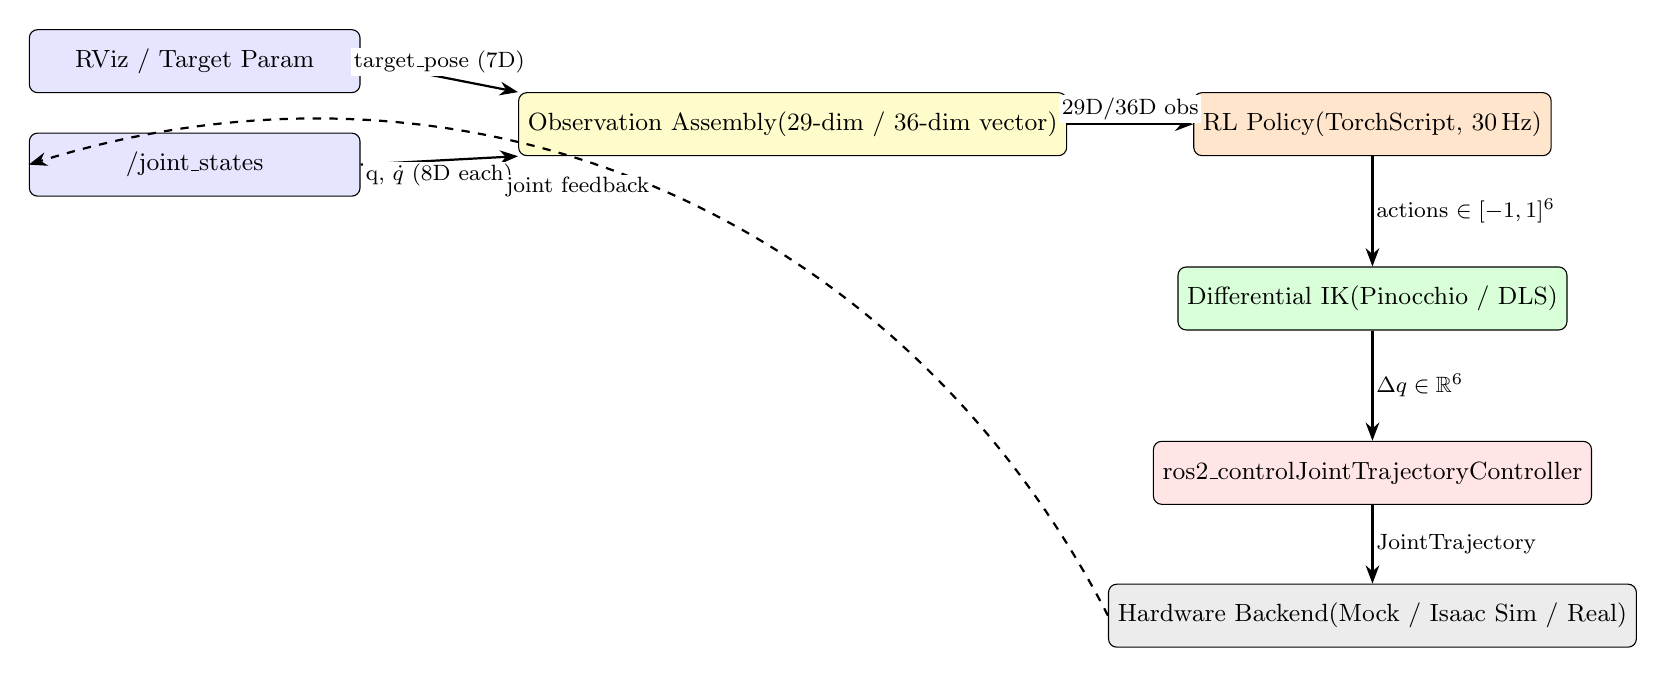
\begin{tikzpicture}[
  node distance = 5mm and 14mm,
  box/.style = {rectangle, draw, rounded corners=3pt, minimum width=42mm,
                minimum height=8mm, text centered, font=\small},
  arr/.style = {-Stealth, thick},
  label/.style = {font=\footnotesize, midway, fill=white, inner sep=1pt}
]
  % Input sources
  \node[box, fill=blue!10]  (marker)  {RViz / Target Param};
  \node[box, fill=blue!10, below=of marker]  (joints)  {/joint\_states};

  % Observation assembly
  \node[box, fill=yellow!20, right=20mm of marker, yshift=-8mm] (obs)
        {Observation Assembly\\(29-dim / 36-dim vector)};

  % Policy
  \node[box, fill=orange!20, right=16mm of obs] (policy)
        {RL Policy\\(TorchScript, 30\,Hz)};

  % DLS IK
  \node[box, fill=green!15, below=14mm of policy] (ik)
        {Differential IK\\(Pinocchio / DLS)};

  % ros2_control
  \node[box, fill=red!10, below=14mm of ik] (ctrl)
        {ros2\_control\\JointTrajectoryController};

  % Hardware
  \node[box, fill=gray!15, below=10mm of ctrl] (hw)
        {Hardware Backend\\(Mock / Isaac~Sim / Real)};

  % Arrows
  \draw[arr] (marker.east) -- node[label, above]{target\_pose (7D)} (obs.north west);
  \draw[arr] (joints.east) -- node[label, below]{q, $\dot{q}$ (8D each)} (obs.south west);
  \draw[arr] (obs)   -- node[label, above]{29D/36D obs} (policy);
  \draw[arr] (policy) -- node[label, right]{actions $\in [-1,1]^6$} (ik);
  \draw[arr] (ik)   -- node[label, right]{$\Delta q \in \mathbb{R}^6$} (ctrl);
  \draw[arr] (ctrl)  -- node[label, right]{JointTrajectory} (hw);

  % Feedback arrow
  \draw[arr, dashed, bend right=40] (hw.west) to
        node[label, left, font=\footnotesize]{joint feedback} (joints.west);
\end{tikzpicture}
\caption{End-to-end data flow of the \texttt{sim2real\_node}.}
\label{fig:dataflow}
\end{figure}

\subsection{Observation Space}
\label{ssec:obs}

The package supports two policy configurations with different observation dimensions depending on the task:

\subsubsection{Reach Task (29-Dimensional Observation Space)}
The reach policy receives a 29-dimensional flat observation vector $\mathbf{o}_t^{\text{reach}} \in \mathbb{R}^{29}$ assembled at each 30~Hz control step:

\begin{equation}
  \mathbf{o}_t^{\text{reach}} = \bigl[\,
    \underbrace{\mathbf{q}_t - \mathbf{q}_{\text{def}}}_{\text{8D, pos. rel.}},\;
    \underbrace{\dot{\mathbf{q}}_t}_{\text{8D, velocity}},\;
    \underbrace{\mathbf{p}^*_t}_{\text{7D, pose cmd}},\;
    \underbrace{\mathbf{a}_{t-1}}_{\text{6D, last action}}
  \,\bigr]
  \label{eq:obs_reach}
\end{equation}

where:
\begin{itemize}[nosep]
  \item $\mathbf{q}_t \in \mathbb{R}^8$ — current joint positions (6 arm + 2 gripper carriage joints),
  \item $\mathbf{q}_{\text{def}} \in \mathbb{R}^8$ — default (nominal) joint configuration,
  \item $\dot{\mathbf{q}}_t \in \mathbb{R}^8$ — current joint velocities (rad/s),
  \item $\mathbf{p}^*_t = [x^*, y^*, z^*, q^*_w, q^*_x, q^*_y, q^*_z]^\top \in \mathbb{R}^7$ — desired
        end-effector pose in the base frame, expressed as position and unit quaternion,
  \item $\mathbf{a}_{t-1} \in \mathbb{R}^6$ — previous policy action (raw, unclipped).
\end{itemize}

\subsubsection{Control Panel Switch Task (36-Dimensional Observation Space)}
The switch policy adds the current end-effector pose $\mathbf{p}_t$ to the observation space, yielding a 36-dimensional flat vector $\mathbf{o}_t^{\text{switch}} \in \mathbb{R}^{36}$:

\begin{equation}
  \mathbf{o}_t^{\text{switch}} = \bigl[\,
    \underbrace{\mathbf{q}_t - \mathbf{q}_{\text{def}}}_{\text{8D, pos. rel.}},\;
    \underbrace{\dot{\mathbf{q}}_t}_{\text{8D, velocity}},\;
    \underbrace{\mathbf{p}_t}_{\text{7D, ee pose}},\;
    \underbrace{\mathbf{a}_{t-1}}_{\text{6D, last action}},\;
    \underbrace{\mathbf{p}^*_t}_{\text{7D, pose cmd}}
  \,\bigr]
  \label{eq:obs_switch}
\end{equation}

where $\mathbf{p}_t = [x, y, z, q_w, q_x, q_y, q_z]^\top \in \mathbb{R}^7$ is the current end-effector pose computed in the base frame using forward kinematics.

The default joint configuration $\mathbf{q}_{\text{def}}$ for both tasks is defined as:

\begin{equation}
  \mathbf{q}_{\text{def}} = \bigl[\,0,\;\tfrac{\pi}{3},\;\tfrac{\pi}{6},\;\tfrac{\pi}{5},\;0,\;0,\;0,\;0\,\bigr]^\top
  \label{eq:qdef}
\end{equation}

\subsection{Action Space and Differential Inverse Kinematics}
\label{ssec:action}

The policy outputs a 6-dimensional action $\mathbf{a}_t \in [-1, 1]^6$, clipped after
inference. The first 3 components represent translational end-effector velocity
increments; the last 3 represent rotational increments:

\begin{equation}
  \boldsymbol{\xi}_t =
  \begin{bmatrix} \Delta \mathbf{p} \\ \Delta \boldsymbol{\omega} \end{bmatrix}
  =
  \begin{bmatrix}
    \alpha_p \cdot \mathbf{a}_{t,1:3} \\
    \alpha_r \cdot \mathbf{a}_{t,4:6}
  \end{bmatrix}
  \label{eq:delta_pose}
\end{equation}

where $\alpha_p$ and $\alpha_r$ are velocity-scaling coefficients (node-dependent,
see Table~\ref{tab:nodes}).

Given the arm Jacobian $\mathbf{J}_{\text{arm}} \in \mathbb{R}^{6 \times 6}$ evaluated
at the current configuration $\mathbf{q}_t$ via Pinocchio, the joint angle increment
$\Delta \mathbf{q}_{\text{arm}}$ is computed using the Damped Least Squares (DLS)
pseudo-inverse:

\begin{equation}
  \Delta \mathbf{q}_{\text{arm}} =
  \mathbf{J}_{\text{arm}}^\top
  \left(\mathbf{J}_{\text{arm}}\mathbf{J}_{\text{arm}}^\top + \lambda^2 \mathbf{I}_6\right)^{-1}
  \boldsymbol{\xi}_t
  \label{eq:dls}
\end{equation}

with damping coefficient $\lambda = 0.01$. The DLS formulation prevents numerical
instability near kinematic singularities, where the standard Moore--Penrose
pseudo-inverse would produce unbounded joint velocities.

The Jacobian is computed in the \texttt{LOCAL\_WORLD\_ALIGNED} reference frame,
which aligns the linear velocity components with the world frame while keeping
angular velocity expressed locally. The joint indices of the gripper carriage joints
are excluded from $\mathbf{J}_{\text{arm}}$ so that IK is solved only for the 6 arm
revolute joints.

The commanded joint positions are then:
\begin{equation}
  \mathbf{q}_{t+1}^{\text{cmd}} = \mathbf{q}_t + \Delta \mathbf{q}_{\text{arm}}
  \label{eq:q_cmd}
\end{equation}

% ─────────────────────────────────────────────────────────────
\section{Node Descriptions}
\label{sec:nodes}

\subsection{Comparison of Nodes}
\label{ssec:node_compare}

\begin{table}[h]
\centering
\caption{Comparison of the three control modules}
\label{tab:nodes}
\begin{tabularx}{\textwidth}{lXXX}
\toprule
\textbf{Aspect} &
\textbf{\texttt{sim2real\_node}} &
\textbf{\texttt{sim2real\_node\_trapezoidal}} &
\textbf{\texttt{sim2real\_direct}} \\
\midrule
Node type        & ROS~2 node & ROS~2 node & Standalone Python script \\
Controller       & \texttt{JointTrajectoryController} & \texttt{JointGroupPositionController} & Trossen SDK \\
Output topic/API & \texttt{/arm\_controller/joint\_trajectory} & \texttt{/forward\_position\_controller/commands} & \texttt{driver.set\_joint\_positions()} \\
Output msg type  & \texttt{JointTrajectory} & \texttt{Float64MultiArray} & N/A \\
$\alpha_p$ (m/step)  & 0.005 & 0.010 & 0.010 \\
$\alpha_r$ (rad/step) & 0.010 & 0.020 & 0.020 \\
Max translation speed & 0.15\,m/s & 0.30\,m/s & 0.30\,m/s \\
Max rotation speed & 0.30\,rad/s & 0.60\,rad/s & 0.60\,rad/s \\
External pose topic & Enabled & Disabled & N/A \\
Setup complexity & Zero-config & Controller swap required & Direct SDK \\
\bottomrule
\end{tabularx}
\end{table}

\subsection{\texttt{sim2real\_node} — Primary Node}
\label{ssec:sim2real_node}

The primary node implements the full ROS~2 workflow. At initialization:
\begin{enumerate}
  \item The TorchScript policy is loaded via \texttt{torch.jit.load()} and set to evaluation mode.
  \item A subscription to \texttt{/robot\_description} (QoS: \texttt{TRANSIENT\_LOCAL}, depth~1)
        waits for the URDF, which is written to a temporary file and parsed by
        \texttt{pin.buildModelFromUrdf()} to construct the Pinocchio rigid-body model.
  \item A 6-DOF interactive marker is created in the \texttt{base\_link} frame via the
        \texttt{InteractiveMarkerServer} API.
\end{enumerate}

The 30~Hz control timer calls \texttt{control\_loop()}, which:
\begin{enumerate}
  \item On the first iteration: computes FK of the current state and moves the interactive
        marker to that pose to avoid discontinuous motion.
  \item Assembles the 29-dimensional observation vector (Equation~\ref{eq:obs}).
  \item Performs policy inference under \texttt{torch.no\_grad()} context.
  \item Clips actions to $[-1, 1]$ and stores them as $\mathbf{a}_{t-1}$ for the next step.
  \item Runs Pinocchio FK, frame placement update, and Jacobian computation.
  \item Solves the DLS IK (Equation~\ref{eq:dls}).
  \item Publishes a \texttt{JointTrajectory} with one \texttt{JointTrajectoryPoint} containing
        the incremented joint positions.
\end{enumerate}

\paragraph{Trajectory duration design.}
The \texttt{time\_from\_start} of each trajectory point is set to $1.5 \times T_c$
(where $T_c = 1/f_c = 1/30\,\text{s}$), rather than exactly $T_c$. This design
choice prevents the \texttt{JointTrajectoryController} from completing its spline
and entering a stopped state before the next command arrives, which would produce
visible oscillation ("shaking") in the robot's motion.

\subsection{\texttt{sim2real\_node\_trapezoidal} — Alternate Node}
\label{ssec:sim2real_node_trapezoidal}

This node targets the \texttt{JointGroupPositionController}, which applies its own
trapezoidal velocity and acceleration profiles internally. By publishing raw target
positions as \texttt{Float64MultiArray} to \texttt{/forward\_position\_controller/commands},
the node achieves faster, smoother motion at the cost of requiring a controller switch
prior to launch. The velocity scaling factors are doubled compared to the primary node
(Table~\ref{tab:nodes}), reflecting the controller's capacity for smoother interpolation.

\subsection{\texttt{sim2real\_direct} — Standalone Script}
\label{ssec:sim2real_direct}

The standalone script bypasses the ROS~2 middleware entirely and uses the
\texttt{trossen\_arm} Python SDK to communicate with the physical robot at a fixed IP
address (192.168.1.2). The URDF is generated at startup by invoking \texttt{xacro}
as a subprocess. The control loop uses \texttt{time.sleep()} for rate limiting.
This mode is intended for latency-sensitive experiments where ROS~2 overhead is
undesirable.

% ─────────────────────────────────────────────────────────────
\section{Kinematics Engine: Pinocchio}
\label{sec:pinocchio}

All control modules use \texttt{pinocchio}~\cite{carpentier2019pinocchio},
a C++ rigid-body dynamics library with Python bindings, for online kinematics.
The end-effector frame is \texttt{ee\_gripper\_link}. The following operations
are performed at each control step:

\begin{enumerate}
  \item \texttt{pin.forwardKinematics(model, data, q)} — propagate joint positions
        to compute link placements.
  \item \texttt{pin.updateFramePlacements(model, data)} — update the pose of
        named frames (including \texttt{ee\_gripper\_link}).
  \item \texttt{pin.computeJointJacobians(model, data, q)} — compute the
        full geometric Jacobian.
  \item \texttt{pin.getFrameJacobian(\ldots, LOCAL\_WORLD\_ALIGNED)} — extract
        the $6 \times n$ frame Jacobian in the world-aligned local frame.
\end{enumerate}

Only the columns of $\mathbf{J}$ corresponding to the 6 arm joints (indices
\texttt{arm\_idx\_q}) are retained:
\begin{equation}
  \mathbf{J}_{\text{arm}} = \mathbf{J}[:, \texttt{arm\_idx\_q}] \in \mathbb{R}^{6 \times 6}
\end{equation}

% ─────────────────────────────────────────────────────────────
\section{Interactive Marker Interface}
\label{sec:marker}

The desired end-effector pose $\mathbf{p}^*$ can be specified through three channels:

\begin{enumerate}
  \item \textbf{Interactive marker:} A 6-DOF RViz marker (3 translation + 3 rotation
        axes) in the \texttt{base\_link} frame, served by \texttt{InteractiveMarkerServer}.
        Pose feedback directly updates the observation vector at 30~Hz.
  \item \textbf{\texttt{/target\_pose} topic:} Accepts \texttt{geometry\_msgs/PoseStamped}
        messages (enabled in \texttt{sim2real\_node}).
  \item \textbf{\texttt{/goal\_pose} topic:} Alias for \texttt{/target\_pose}
        (enabled in \texttt{sim2real\_node}).
\end{enumerate}

The marker is initialized to the FK-computed end-effector pose on the first control
step, ensuring spatial continuity from the robot's initial configuration.

% ─────────────────────────────────────────────────────────────
\section{Operating Modes and Hardware Backends}
\label{sec:modes}

\begin{table}[h]
\centering
\caption{Hardware backend configuration}
\label{tab:modes}
\begin{tabular}{llll}
\toprule
\textbf{Mode} & \textbf{\texttt{ros2\_control\_hardware\_type}} & \textbf{Additional Arg} & \textbf{Use Case} \\
\midrule
Mock Components & \texttt{mock\_components} & — & RViz testing, debugging \\
Isaac Sim       & \texttt{isaac} & \texttt{use\_sim\_time:=true} & Physics simulation \\
Real Hardware   & \texttt{real} & \texttt{ip\_address:=<IP>} & Physical deployment \\
\bottomrule
\end{tabular}
\end{table}

\subsection{Isaac Sim Clock Synchronization}
\label{ssec:simtime}

When using NVIDIA Isaac Sim as the physics backend, Isaac Sim acts as the master
simulation clock and publishes to the \texttt{/clock} topic. All ROS~2 nodes must
be launched with \texttt{use\_sim_time:=true} to avoid timestamp inconsistencies
such as \texttt{TF\_OLD\_DATA} errors, which would corrupt the TF tree lookup for
tracking error logging.

The \texttt{/robot\_description} subscription uses \texttt{TRANSIENT\_LOCAL} QoS
durability, ensuring the node receives the URDF even if it subscribes after the
publisher has already latched the message.

% ─────────────────────────────────────────────────────────────
\section{Tracking Error Logging}
\label{sec:tracking}

Every second (every $f_c = 30$ control steps), the node looks up the transform from
\texttt{base\_link} to \texttt{ee\_gripper\_link} via \texttt{tf2\_ros.Buffer} and
logs:

\begin{itemize}[nosep]
  \item Target pose: $[x^*, y^*, z^*, q^*_w, q^*_x, q^*_y, q^*_z]$
  \item Actual pose: $[x, y, z, q_w, q_x, q_y, q_z]$ from TF
  \item Positional error: $[\Delta x, \Delta y, \Delta z] = \mathbf{p}^* - \mathbf{p}$
  \item Quaternion error: component-wise difference
\end{itemize}

The quaternion double-cover ambiguity ($\mathbf{q}$ and $-\mathbf{q}$ represent
the same rotation) is handled by negating the actual quaternion if
$\mathbf{q}^* \cdot \mathbf{q} < 0$.

% ─────────────────────────────────────────────────────────────
\section{Software Dependencies}
\label{sec:deps}

\begin{table}[h]
\centering
\caption{Software dependencies of \texttt{trossen\_sim2real\_ros}}
\label{tab:deps}
\begin{tabular}{lll}
\toprule
\textbf{Dependency} & \textbf{Category} & \textbf{Role} \\
\midrule
\texttt{rclpy}                    & ROS~2      & Python client library \\
\texttt{sensor\_msgs}             & ROS~2      & \texttt{JointState} message \\
\texttt{trajectory\_msgs}         & ROS~2      & \texttt{JointTrajectory} message \\
\texttt{geometry\_msgs}           & ROS~2      & \texttt{PoseStamped} message \\
\texttt{visualization\_msgs}      & ROS~2      & Interactive marker messages \\
\texttt{interactive\_markers}     & ROS~2      & Interactive marker server \\
\texttt{tf2\_ros}                 & ROS~2      & TF2 transform lookup \\
\texttt{torch}                    & Python     & TorchScript policy inference \\
\texttt{pinocchio}                & Python     & FK and Jacobian computation \\
\texttt{numpy}                    & Python     & Numerical computation \\
\texttt{trossen\_arm}             & Python SDK & Direct hardware communication \\
\texttt{ros2\_control}            & ROS~2      & Hardware abstraction layer \\
\texttt{ros2\_controllers}        & ROS~2      & Trajectory / position controllers \\
\texttt{topic\_based\_ros2\_control} & ROS~2   & Isaac Sim topic bridge \\
\bottomrule
\end{tabular}
\end{table}

% ─────────────────────────────────────────────────────────────
\section{Key Design Decisions}
\label{sec:design}

\paragraph{1. Temporal action history in observation.}
Feeding the previous action $\mathbf{a}_{t-1}$ back into the observation vector
provides the policy with a one-step history without requiring a recurrent
architecture. This improves temporal consistency and reduces jerk, at the cost
of one additional observation dimension.

\paragraph{2. Trajectory duration factor of 1.5$\times$.}
Setting \texttt{time\_from\_start} to $1.5 \times T_c$ rather than $T_c$ ensures
that the \texttt{JointTrajectoryController}'s internal spline interpolator is still
\emph{in progress} when the next command arrives. This prevents the stop-and-restart
artifact (visible as high-frequency oscillation) that occurs when the spline endpoint
is reached before a new command.

\paragraph{3. Lazy Pinocchio model initialization.}
The kinematic model is built upon receipt of \texttt{/robot\_description} rather
than at node construction. This decouples the node from the launch order of dependent
packages and enables robust operation across all three hardware modes.

\paragraph{4. Damping coefficient $\lambda = 0.01$.}
The DLS damping value provides a balance between accuracy in non-singular
configurations and stability near singularities. A smaller $\lambda$ yields higher
accuracy at the risk of joint velocity divergence; a larger $\lambda$ over-damps
the solution.

\paragraph{5. Interactive marker initialized from FK.}
Rather than placing the marker at a static default pose, the node computes forward
kinematics of the actual initial configuration and positions the marker there. This
prevents a sudden commanded displacement on the first control step.

\paragraph{6. Action clipping to $[-1, 1]$.}
Hard clipping provides a safety bound on per-step joint displacement regardless
of policy output distribution, acting as a first-layer safety mechanism independent
of the DLS scaling factors.

% ─────────────────────────────────────────────────────────────
\section{Conclusion}
\label{sec:conclusion}

The \texttt{trossen\_sim2real\_ros} package provides a clean, modular implementation
of the sim-to-real deployment pipeline for RL-based reach tasks on the Trossen
WidowX~AI arm. By separating the policy inference, kinematics, and hardware
interface layers, the package supports seamless switching between simulation and
physical hardware without code modification. The Damped Least Squares Differential
IK approach, combined with Pinocchio's efficient Jacobian computation, ensures
real-time performance at 30~Hz while maintaining singularity robustness. The
interactive 6-DOF marker interface provides a practical tool for real-time task
specification during experiments.

% ─────────────────────────────────────────────────────────────
\begin{thebibliography}{9}

\bibitem{carpentier2019pinocchio}
J.~Carpentier, G.~Saurel, G.~Buondonno, J.~Mirabel, F.~Lamiraux, O.~Stasse,
and N.~Mansard,
``The Pinocchio C++ library: A fast and flexible implementation of rigid body
dynamics algorithms and their analytical derivatives,''
in \textit{IEEE International Symposium on System Integration (SII)}, 2019.

\bibitem{rudin2022learning}
N.~Rudin, D.~Hoeller, P.~Reist, and M\_Hutter,
``Learning to walk in minutes using massively parallel deep reinforcement learning,''
in \textit{Conference on Robot Learning (CoRL)}, 2022.

\bibitem{isaaclab}
NVIDIA Corporation,
``Isaac Lab: A Unified and Modular Reinforcement Learning Framework for Robot
Learning,''
\url{https://isaac-sim.github.io/IsaacLab/}, 2024.

\bibitem{ros2control}
B.~Aceituno-Cabezas, C\_Mastalli, H\_Dai, M\_Focchi, A\_Radulescu, D\_G\_Caldwell,
J\_Carpentier, M\_Vijayakumar, W\_Bosworth, and C\_Semini,
``Simultaneous contact, gait, and motion planning for robust multilegged locomotion
via mixed-integer convex optimization,''
\textit{IEEE Robotics and Automation Letters}, 2017.

\end{thebibliography}

\end{document}
